\documentclass[12pt]{article}
\usepackage{times} 			% use Times New Roman font

\usepackage[margin=1in]{geometry}   % sets 1 inch margins on all sides
\usepackage{hyperref}               % for URL formatting
\usepackage[pdftex]{graphicx}       % So includegraphics will work
\setlength{\parskip}{1em}           % skip 1em between paragraphs
\usepackage{indentfirst}            % indent the first line of each paragraph
\usepackage{datetime}
\usepackage[small, bf]{caption}
\usepackage{listings}               % for code listings
\usepackage{xcolor}                 % for styling code
\usepackage{multirow}
\usepackage{longtable}
\usepackage{multirow}
\usepackage{float}
%New colors defined below
\definecolor{backcolour}{RGB}{246, 246, 246}   % 0xF6, 0xF6, 0xF6
\definecolor{codegreen}{RGB}{16, 124, 2}       % 0x10, 0x7C, 0x02
\definecolor{codepurple}{RGB}{170, 0, 217}     % 0xAA, 0x00, 0xD9
\definecolor{codered}{RGB}{154, 0, 18}         % 0x9A, 0x00, 0x12

%Code listing style named "gcolabstyle" - matches Google Colab
\lstdefinestyle{gcolabstyle}{
  basicstyle=\ttfamily\small,
  backgroundcolor=\color{backcolour},   
  commentstyle=\itshape\color{codegreen},
  keywordstyle=\color{codepurple},
  stringstyle=\color{codered},
  numberstyle=\ttfamily\footnotesize\color{darkgray}, 
  breakatwhitespace=false,         
  breaklines=true,                 
  captionpos=b,                    
  keepspaces=true,                 
  numbers=left,                    
  numbersep=5pt,                  
  showspaces=false,                
  showstringspaces=false,
  showtabs=false,                  
  tabsize=2
}

\lstset{style=gcolabstyle}      %set gcolabstyle code listing

% to make long URIs break nicely
\makeatletter
\g@addto@macro{\UrlBreaks}{\UrlOrds}
\makeatother

% for fancy page headings
\usepackage{fancyhdr}
\setlength{\headheight}{13.6pt} % to remove fancyhdr warning
\pagestyle{fancy}
\fancyhf{}
\rhead{\small \thepage}
\lhead{\small HW6, Adeniran}  % EDIT THIS, REPLACE # with HW number
\chead{\small CS 532, Spring 2021} 

%-------------------------------------------------------------------------
\begin{document}

\begin{centering}
{\large\textbf{HW6 - Analyzing Disinformation Domains}}\\ % EDIT THIS
                                % REPLACE # with HW num and ADD title
Adeniran Adeniyi\\                     % EDIT THIS
Sunday, April 4, 2021 by 11:59pm\\                      % EDIT THIS
\end{centering}

%-------------------------------------------------------------------------

% The * after \section just says to not number the sections
%----------------------------Q1111111111111111111111111111111111

\section*{Q1}
\emph{Datasets D1 and D2 include the number of tweets that each domain was shared in (found in the last column/field of the dataset).\\ \\
For each of D1 and D2, what were the top 10 domains in terms of tweets? Which ones are no longer live? Load the main web-page in your web browser. How would you classify the domain? Show this information in a table like the one below, sorted by number of tweets. You should have 2 tables, one for D1 and one for D2.}
\subsection*{\color{blue}{Answer}}
\lstinputlisting[language=Python,caption=question1.py, label=Q1a:import,firstnumber=1,firstline=1,lastline=73]{question1.py}


\begin{center}
\begin{longtable}{|l|l|l|l|}
\caption{Top 10 High Number of Tweets Domains (Processed D1)} \label{tab:long} \\

\hline \multicolumn{1}{|c|}{\textbf{Domain}} & \multicolumn{1}{|c|}{\textbf{Tweets}}  & \multicolumn{1}{|c|}{\textbf{Media}} &  \multicolumn{1}{|c|}{\textbf{Status}}  \\ \hline 
\endfirsthead

\multicolumn{2}{c}%
{{\bfseries \tablename\ \thetable{} -- continued from previous page}} \\
\hline  \multicolumn{1}{|c|}{\textbf{Domain}} & \multicolumn{1}{|c|}{\textbf{Tweets}}  & \multicolumn{1}{|c|}{\textbf{Media}} &  \multicolumn{1}{|c|}{\textbf{Status}}  \\ \hline 
\endhead

\hline \multicolumn{2}{|c|}{{Continued on next page}} \\ \hline
\endfoot

\hline \hline
\endlastfoot
therealstrategy.com  & 7113   & Alternative Media & not live \\
infowars.com         & 1741   & Alternative Media & live     \\
newsbusters.org      & 1217   & Alternative Media & live     \\
washingtonpost.com   & 1108   & MSM               & live     \\
nodisinfo.com        & 774    & Alternative Media & not live \\
nytimes.com          & 759    & MSM               & live     \\
veteranstoday.com    & 586    & Alternative Media & live     \\
beforeitsnews.com    & 580    & Alternative Media & live     \\
rawstory.com         & 308    & Alternative Media & live     \\
hoax.trendolizer.com & 299    & fact checker      & live \\
\end{longtable}
\end{center}


\begin{center}
\begin{longtable}{|l|l|l|l|}
\caption{Top 10 High Number of Tweets Domains (Processed D2)} \label{tab:long} \\

\hline \multicolumn{1}{|c|}{\textbf{Domain}} & \multicolumn{1}{|c|}{\textbf{Tweets}}  & \multicolumn{1}{|c|}{\textbf{Media}} &  \multicolumn{1}{|c|}{\textbf{Status}}  \\ \hline 
\endfirsthead

\multicolumn{2}{c}%
{{\bfseries \tablename\ \thetable{} -- continued from previous page}} \\
\hline  \multicolumn{1}{|c|}{\textbf{Domain}} & \multicolumn{1}{|c|}{\textbf{Tweets}}  & \multicolumn{1}{|c|}{\textbf{Media}} &  \multicolumn{1}{|c|}{\textbf{Status}}  \\ \hline 
\endhead

\hline \multicolumn{2}{|c|}{{Continued on next page}} \\ \hline
\endfoot

\hline \hline
\endlastfoot
21stcenturywire.com & 3088  & Alternative Media            & live   \\
clarityofsignal.com & 2352  & Not Found(Alternative Media) & live   \\
rt.com              & 1598  & Foreign Government Media     & live   \\
newsweek.com        & 1249  & Not Found(MSM)               & live   \\
alternet.org        & 1221  & Not Found(Alternative Media) & live   \\
sputniknews.com     & 1076  & Foreign Government Media     & live   \\
mintpressnews.com   & 919   & Not Found(Alternative Media) & live   \\
cnn.com             & 756   & MSM                          & live   \\
globalresearch.ca   & 724   & Alternative Media            & live   \\
theantimedia.org    & 682   & Alternative Media            & live  
\end{longtable}
\end{center}
\subsection*{Discussion}

\emph{For D1processed I read the D1.csv file in a pandas dataFrame and was able to easily to sort the data according to The number of Tweets in Highest to lowest. As for processed D2 I did the same thing but I read in D2.csv and also compared the data with D1.csv to obtain the Media Values. Those values that are not found shows not found and what i manually classified them. I also manual checked the website on the browser to check if the where active website.}

\section*{Q2}
\emph{Compare the amount of overlap between the three datasets.
Generate the following datasets:}
    \begin{itemize}
        \item a. domains that are present in both D1 and D2
        \item b. domains that are present in both D2 and D3
        \item c. domains that are present in both D1 and D3
        \item d. domains that are present in all three datasets
    \end{itemize}
\subsection*{\color{blue}{Answer}}
\lstinputlisting[language=Python,caption=overlap.py for question 2, label=Q1a:import,firstnumber=1,firstline=1,lastline=63]{overlap.py}
\begin{center}
\begin{longtable}{|l|}
\caption{Domains that are present in both D1 and D2 (gotten from finalA)} \label{tab:long} \\

\hline \multicolumn{1}{|c|}{\textbf{Domain}}  \\ \hline 
\endfirsthead

\multicolumn{1}{c}%
{{\bfseries \tablename \thetable{} -- continued from previous page}} \\
\hline  \multicolumn{1}{|c|}{\textbf{Domain}}  \\ \hline 
\endhead

\hline \multicolumn{1}{|c|}{{Continued on next page}} \\ \hline
\endfoot

\hline \hline
\endlastfoot
rt.com                    \\
breitbart.com             \\
theeventchronicle.com     \\
therussophile.org         \\
themillenniumreport.com   \\
beforeitsnews.com         \\
cbsnews.com               \\
thefreethoughtproject.com \\
veteranstoday.com         \\
theintercept.com          \\
theguardian.com           \\
21stcenturywire.com       \\
infowars.com              \\
thedailybeast.com         \\
heavy.com                 \\
blacklistednews.com       \\
presstv.com               \\
dcclothesline.com         \\
theantimedia.org          \\
upi.com                   \\
investmentwatchblog.com   \\
dailymail.co.uk           \\
mirror.co.uk              \\
nydailynews.com           \\
fellowshipoftheminds.com  \\
thetruthseeker.co.uk      \\
abovetopsecret.com        \\
cnn.com                   \\
worldtruth.tv             \\
sputniknews.com           \\
lewrockwell.com           \\
nytimes.com               \\
intellihub.com            \\
thedailysheeple.com       \\
globalresearch.ca         \\
foxnews.com               \\
thestar.com               \\
activistpost.com          \\
nbcnews.com  
\end{longtable}
\end{center}


\begin{center}
\begin{longtable}{|l|}
\caption{Domains that are present in both D2 and D3 (gotten from finalB.csv)} \label{tab:long} \\

\hline \multicolumn{1}{|c|}{\textbf{Domain}}  \\ \hline 
\endfirsthead

\multicolumn{1}{c}%
{{\bfseries \tablename \thetable{} -- continued from previous page}} \\
\hline  \multicolumn{1}{|c|}{\textbf{Domain}}  \\ \hline 
\endhead

\hline \multicolumn{1}{|c|}{{Continued on next page}} \\ \hline
\endfoot

\hline \hline
\endlastfoot
activistpost.com          \\
beforeitsnews.com         \\
breitbart.com             \\
collective-evolution.com  \\
dcclothesline.com         \\
gellerreport.com          \\
humansarefree.com         \\
infowars.com              \\
intellihub.com            \\
ronpaulinstitute.org      \\
sott.net                  \\
thewashingtonstandard.com \\
worldtruth.tv             \\
21stcenturywire.com       \\
davidicke.com             \\
off-guardian.org          \\
presstv.com               \\
ukcolumn.org              \\
rubikon.news              \\
globalresearch.ca         \\
theduran.com 
\end{longtable}
\end{center}


\begin{center}
\begin{longtable}{|l|}
\caption{Domains that are present in both D1 and D3 (gotten from finalC.csv)} \label{tab:long} \\

\hline \multicolumn{1}{|c|}{\textbf{Domain}}  \\ \hline 
\endfirsthead

\multicolumn{1}{c}%
{{\bfseries \tablename \thetable{} -- continued from previous page}} \\
\hline  \multicolumn{1}{|c|}{\textbf{Domain}}  \\ \hline 
\endhead

\hline \multicolumn{1}{|c|}{{Continued on next page}} \\ \hline
\endfoot

\hline \hline
\endlastfoot
activistpost.com    \\
beforeitsnews.com   \\
breitbart.com       \\
dcclothesline.com   \\
infowars.com        \\
intellihub.com      \\
wakingtimes.com     \\
worldtruth.tv       \\
zerohedge.com       \\
21stcenturywire.com \\
presstv.com         \\
globalresearch.ca  
\end{longtable}
\end{center}


\begin{center}
\begin{longtable}{|l|}
\caption{domains that are present in all three datasets (gotten from finalD.csv)} \label{tab6:long} \\

\hline \multicolumn{1}{|c|}{\textbf{Domain}}  \\ \hline 
\endfirsthead

\multicolumn{1}{c}%
{{\bfseries \tablename \thetable{} -- continued from previous page}} \\
\hline  \multicolumn{1}{|c|}{\textbf{Domain}}  \\ \hline 
\endhead

\hline \multicolumn{1}{|c|}{{Continued on next page}} \\ \hline
\endfoot

\hline \hline
\endlastfoot
activistpost.com    \\
beforeitsnews.com   \\
breitbart.com       \\
dcclothesline.com   \\
infowars.com        \\
intellihub.com      \\
worldtruth.tv       \\
21stcenturywire.com \\
presstv.com         \\
globalresearch.ca  
\end{longtable}


\end{center}
\subsection*{Discussion}
\emph{I created a function called compareThisB(lowerCase,upperCase) to handle all the process for comparisons, for a,b,c,and d. This functions takes the two parameters. The second parameters get converted in all lower case before comparisons. }


\section*{Q3}
Collect at least 200 tweets that contain links from domains that appear in both D3 and one of the other datasets (so, dataset b or dataset c from Q2).

\subsection*{\color{blue}{Answer}}
\lstinputlisting[language=Python,caption=collecting-tweet.py used for collecting tweet info per domain, label=Q3:import,firstnumber=1,firstline=1,lastline=52]{collect-tweet.py}
\lstinputlisting[language=Python,caption=processing.py for question 3 and 4 data processing, label=Q3:import,firstnumber=1,firstline=1,lastline=113]{processing.py}
\begin{figure}[H]
            \centering
            % trim and clip are used to crop the image, trim=left bottom right top
            % width sets max width, height will be scaled appropriately
            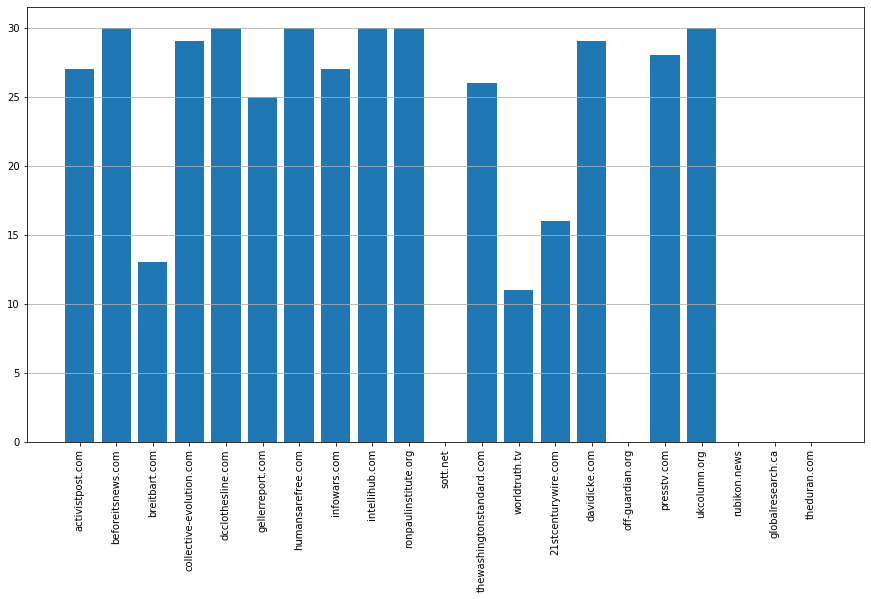
\includegraphics[trim=0 0 0 0, clip, width=\textwidth] {barchar3.png}
            \caption{ a bar chart showing the number of tweets for each domain}
            \label{fig:Q2Ans}
        \end{figure}
\subsection*{Discussion}
\emph{Collect-tweet.py does the processing of collecting the tweet information using the lists of domain created in Question 2B(Q2/finalB.csv).\\ \\Using the processing.py script, I read the csvjson.json file into a pandas dataFrame, and using the dataFrame I was able to process the information to answer the questions below}
    \begin{itemize}
        \item How many tweets did you gather?\\ \\ I was able to gather 450 tweets, I read the json converted csvjson.json file into pandas dataFrame. Using the .shape[0] gets the size of the dataFrame
        \item What was the time range of the tweets you gathered?\\ \\ The time range is from 2021-04-04 22:21:48 to 2021-03-27 20:25:22
        \item How many different accounts posted those tweets?\\ \\ There are 306 different users, using the unique function to get all unique values in a column. It get the total unique screen names from the data I gathered(450).
        
        \item For those domains that had at least one tweet, how many tweets did you discover for each domain? To answer this question, create a bar chart showing the number of tweets for each domain.
        Answer in Table \ref{fig:Q2Ans}
    \end{itemize}
\section*{Q4}
Compare the number of tweets per domain from Q3 with the information in D1 and D2. What were the top 10 shared domains from Q3? How does this compare with the top 10 shared domains in D1 and D2 (from Q1)?
For those domains that had at least one tweet, how many accounts were posting links for each domain?

To answer this question, create a bar chart showing the number of accounts for each domain.
\subsection*{\color{blue}{Answer}}
\lstinputlisting[language=Python,caption=processing.py for question 3 and 4 data processing, label=Q3:import,firstnumber=1,firstline=1,lastline=113]{processing.py}
\begin{center}
\begin{longtable}{|l|l|}
\caption{The top 10 shared domains from Q3}
\label{tab7:long} \\

\hline \multicolumn{1}{|c|}{\textbf{Domain}} & \multicolumn{1}{|c|}{\textbf{Number Of Tweets}}  \\ \hline 
\endfirsthead

\multicolumn{1}{c}%
{{\bfseries \tablename \thetable{} -- continued from previous page}} \\
\hline  \multicolumn{1}{|c|}{\textbf{Domain}}  & \multicolumn{1}{|c|}{\textbf{Number Of Tweets}}  \\ \hline 
\endhead

\hline \multicolumn{1}{|c|}{{Continued on next page}} \\ \hline
\endfoot

\hline \hline
\endlastfoot
ronpaulinstitute.org     & 30    \\
humansarefree.com        & 30    \\
beforeitsnews.com        & 30    \\
intellihub.com           & 30    \\
ukcolumn.org             & 30    \\
dcclothesline.com        & 30    \\
collective-evolution.com & 29    \\
davidicke.com            & 29    \\
presstv.com              & 28    \\
infowars.com             & 27     
\end{longtable}
\end{center}

\begin{center}
\begin{longtable}{|l|l|l|l|}
\caption{Top 10 High Number of Tweets Domains (Processed D1)} \label{tab8:long} \\

\hline \multicolumn{1}{|c|}{\textbf{Domain}} & \multicolumn{1}{|c|}{\textbf{Tweets}}  & \multicolumn{1}{|c|}{\textbf{Media}} &  \multicolumn{1}{|c|}{\textbf{Status}}  \\ \hline 
\endfirsthead

\multicolumn{2}{c}%
{{\bfseries \tablename\ \thetable{} -- continued from previous page}} \\
\hline  \multicolumn{1}{|c|}{\textbf{Domain}} & \multicolumn{1}{|c|}{\textbf{Tweets}}  & \multicolumn{1}{|c|}{\textbf{Media}} &  \multicolumn{1}{|c|}{\textbf{Status}}  \\ \hline 
\endhead

\hline \multicolumn{2}{|c|}{{Continued on next page}} \\ \hline
\endfoot

\hline \hline
\endlastfoot
therealstrategy.com  & 7113   & Alternative Media & not live \\
infowars.com         & 1741   & Alternative Media & live     \\
newsbusters.org      & 1217   & Alternative Media & live     \\
washingtonpost.com   & 1108   & MSM               & live     \\
nodisinfo.com        & 774    & Alternative Media & not live \\
nytimes.com          & 759    & MSM               & live     \\
veteranstoday.com    & 586    & Alternative Media & live     \\
beforeitsnews.com    & 580    & Alternative Media & live     \\
rawstory.com         & 308    & Alternative Media & live     \\
hoax.trendolizer.com & 299    & fact checker      & live \\
\end{longtable}
\end{center}


\begin{center}
\begin{longtable}{|l|l|l|l|}
\caption{Top 10 High Number of Tweets Domains (Processed D2)} \label{tab9:long} \\

\hline \multicolumn{1}{|c|}{\textbf{Domain}} & \multicolumn{1}{|c|}{\textbf{Tweets}}  & \multicolumn{1}{|c|}{\textbf{Media}} &  \multicolumn{1}{|c|}{\textbf{Status}}  \\ \hline 
\endfirsthead

\multicolumn{2}{c}%
{{\bfseries \tablename\ \thetable{} -- continued from previous page}} \\
\hline  \multicolumn{1}{|c|}{\textbf{Domain}} & \multicolumn{1}{|c|}{\textbf{Tweets}}  & \multicolumn{1}{|c|}{\textbf{Media}} &  \multicolumn{1}{|c|}{\textbf{Status}}  \\ \hline 
\endhead

\hline \multicolumn{2}{|c|}{{Continued on next page}} \\ \hline
\endfoot

\hline \hline
\endlastfoot
21stcenturywire.com & 3088  & Alternative Media            & live   \\
clarityofsignal.com & 2352  & Not Found(Alternative Media) & live   \\
rt.com              & 1598  & Foreign Government Media     & live   \\
newsweek.com        & 1249  & Not Found(MSM)               & live   \\
alternet.org        & 1221  & Not Found(Alternative Media) & live   \\
sputniknews.com     & 1076  & Foreign Government Media     & live   \\
mintpressnews.com   & 919   & Not Found(Alternative Media) & live   \\
cnn.com             & 756   & MSM                          & live   \\
globalresearch.ca   & 724   & Alternative Media            & live   \\
theantimedia.org    & 682   & Alternative Media            & live  
\end{longtable}
\end{center}

\begin{figure}[H]
            \centering
            % trim and clip are used to crop the image, trim=left bottom right top
            % width sets max width, height will be scaled appropriately
            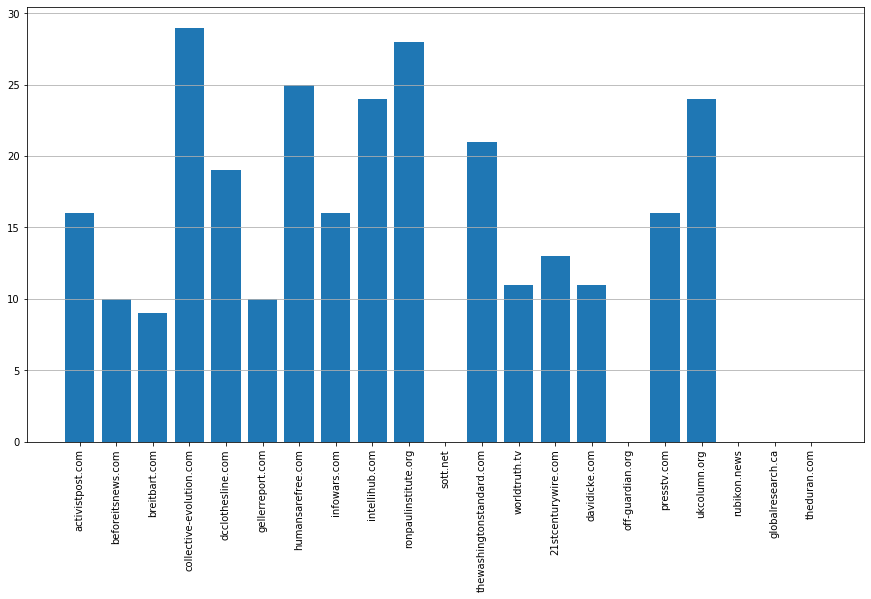
\includegraphics[trim=0 0 0 0, clip, width=\textwidth] {barchar4.png}
            \caption{ a bar chart showing the number of accounts for each domain}
            \label{fig:Q4Ans}
        \end{figure}
\subsection*{Discussion}
\emph{I used processing.py to get the questions answered, more details are in processing.py}
\emph{I followed this instructions}
    \begin{itemize}
        \item Compare the number of tweets per domain from Q3 with the information in D1 and D2. I used the code in processing  
        I compared the  from Q4/tweetPerDomain folders
        \item What were the top 10 shared domains from Q3? \\ Answer in Table \ref{tab7:long}
        \item How does this compare with the top 10 shared domains in D1 and D2 (from Q1)?  \\ \\ They had these domains in common: \\
        beforeitsnews.com  (in D1) \\
        infowars.com  (in D1)   \\
        Nothing at all was common in D2
         \item For those domains that had at least one tweet, how many accounts were posting links for each domain?To answer this question, create a bar chart showing the number of accounts for each domain.
        \\ \\ Answer in Figure \ref{fig:Q4Ans}
    \end{itemize}
\section*{Q5}
\emph{There have been several online games created to educate people about disinformation and how it spreads on social media. Play one of the games at either https://www.getbadnews.com or https://goviralgame.com. Write a paragraph about your experience and some lessons you learned by playing the game. Take some screenshots as you play to include in your report.}
\subsection*{\color{blue}{Answer}}
\begin{figure}[H]
            \centering
            % trim and clip are used to crop the image, trim=left bottom right top
            % width sets max width, height will be scaled appropriately
            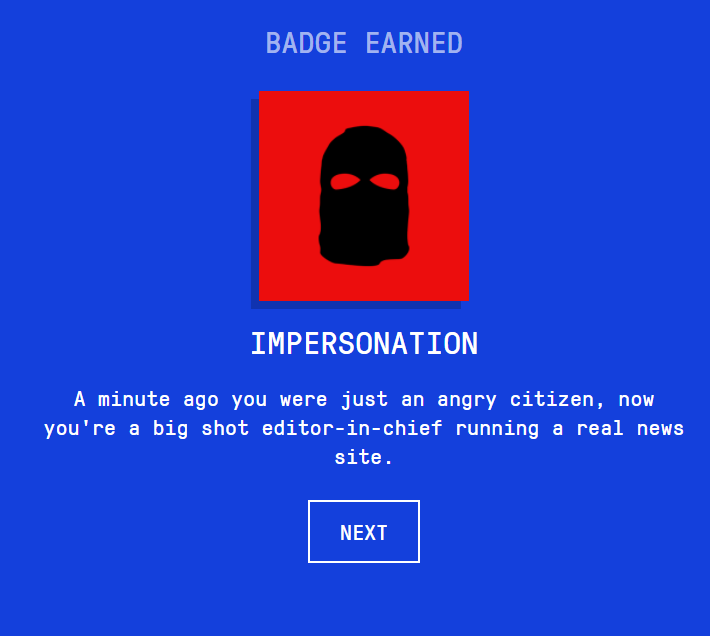
\includegraphics[trim=0 0 0 0, clip, width=\textwidth] {firstBadge.PNG}
            \caption{ a bar chart showing the number of accounts for each domain}
            \label{fig:1}
\end{figure}
\begin{figure}[H]
            \centering
            % trim and clip are used to crop the image, trim=left bottom right top
            % width sets max width, height will be scaled appropriately
            \includegraphics[trim=0 0 0 0, clip, width=\textwidth] {secondBadge.PNG}
            \caption{ a bar chart showing the number of accounts for each domain}
            \label{fig:2}
\end{figure}
\begin{figure}[H]
            \centering
            % trim and clip are used to crop the image, trim=left bottom right top
            % width sets max width, height will be scaled appropriately
            \includegraphics[trim=0 0 0 0, clip, width=\textwidth] {thirdBadge.PNG}
            \caption{ a bar chart showing the number of accounts for each domain}
            \label{fig:3}
\end{figure}
\begin{figure}[H]
            \centering
            % trim and clip are used to crop the image, trim=left bottom right top
            % width sets max width, height will be scaled appropriately
            
\includegraphics[trim=0 0 0 0, clip, width=\textwidth] {fourthbadge.PNG}
            \caption{ a bar chart showing the number of accounts for each domain}
            \label{fig:4}
\end{figure}
\begin{figure}[H]
            \centering
            % trim and clip are used to crop the image, trim=left bottom right top
            % width sets max width, height will be scaled appropriately
            \includegraphics[trim=0 0 0 0, clip, width=\textwidth] {fifthBadge.PNG}
            \caption{ a bar chart showing the number of accounts for each domain}
            \label{fig:5}
\end{figure}
\begin{figure}[H]
            \centering
            % trim and clip are used to crop the image, trim=left bottom right top
            % width sets max width, height will be scaled appropriately
            \includegraphics[trim=0 0 0 0, clip, width=\textwidth] {sixthBadge.PNG}
            \caption{ a bar chart showing the number of accounts for each domain}
            \label{fig:6}
\end{figure}
\begin{figure}[H]
            \centering
            % trim and clip are used to crop the image, trim=left bottom right top
            % width sets max width, height will be scaled appropriately
            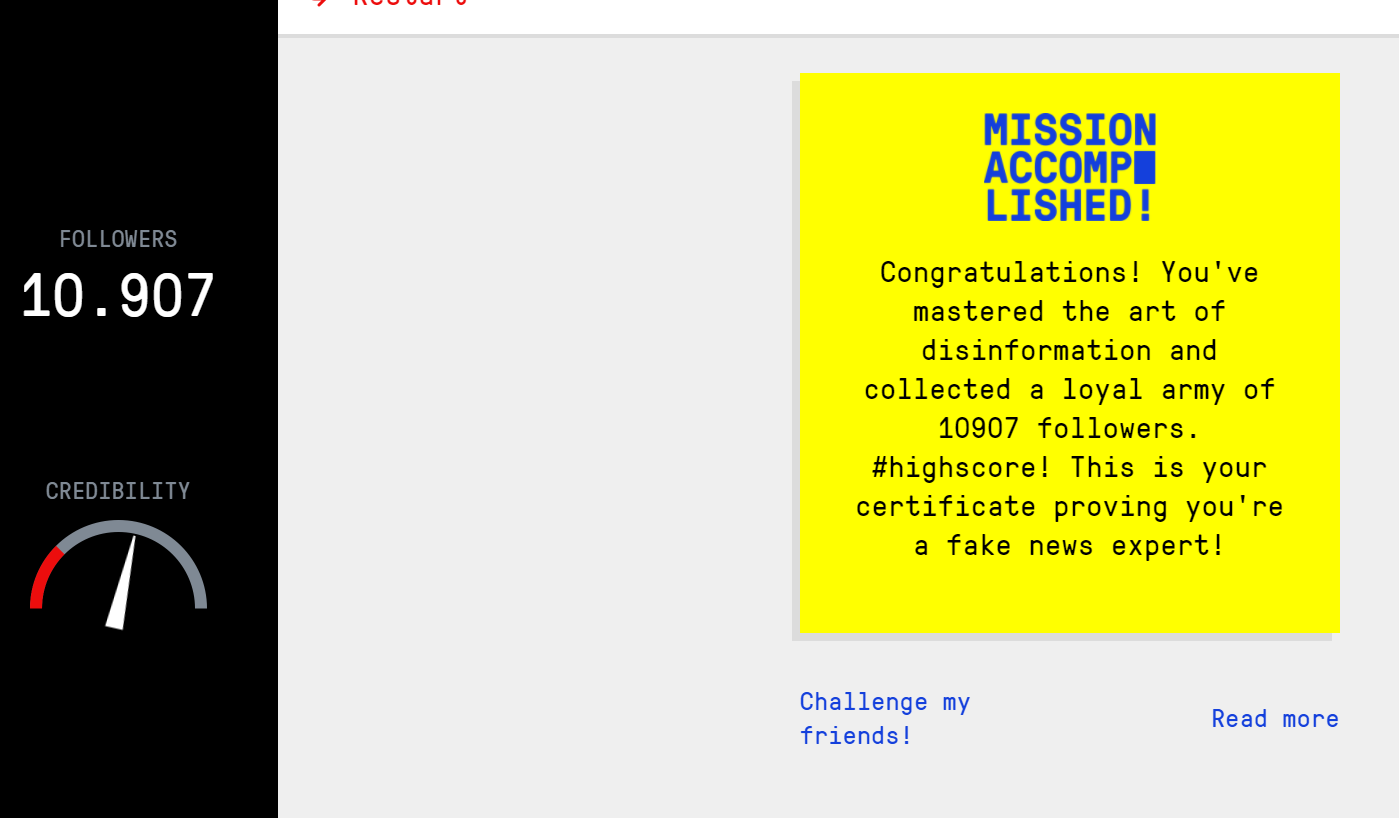
\includegraphics[trim=0 0 0 0, clip, width=\textwidth] {final.PNG}
            \caption{ a bar chart showing the number of accounts for each domain}
            \label{fig:7}
\end{figure}

\subsection*{Discussion}
\emph{I used https://www.getbadnews.com/ to play the came and was able to earn the above badges below:}
    \begin{itemize}
        \item Impersonation in Figure \ref{fig:1} (Impersonating someone else and disguising myself as a credible news source which was highly effective in increase my followers)
        \item Emotion in Figure \ref{fig:2} (Playing to people's emotion out of fear, anger or compassing was a great tool for spreading my messages)
        \item Polarization in Figure \ref{fig:3} (By finding existing grievance and blowing them out of proportion, drove people apart and made think a story is much more important that it really was.)
        \item Conspiracy in Figure \ref{fig:4}(I can use people's desires for the 'truth' as a tool to lure them into my band of followers)
        \item Discredit in Figure \ref{fig:5}(When someone is attacking my credibility i strike back. I do not apologize nor do I play nice and above all I do not retreat!)
        \item Trolling in Figure \ref{fig:6} ( Is a tool that evokes an emotional response such as anger, irritation or sadness. Dont hold back: your opponent's tears are your followers' mead!)
        \item The final score was 10907 followers.in Figure \ref{fig:7}
    \end{itemize}


\section*{References}
\begin{itemize}
    \item {\url{https://www.datacamp.com/community/tutorials/pandas-read-csv}}
     \item {\url{https://pandas.pydata.org/docs/reference/api/pandas.DataFrame.sort_values.html}}
     \item {\url{https://stackoverflow.com/questions/12021754/how-to-slice-a-pandas-data-frame-by-position}}
     \item {\url{https://pandas.pydata.org/pandas-docs/stable/reference/api/pandas.DataFrame.rename.html}}
     \item {\url{https://pandas.pydata.org/docs/reference/api/pandas.DataFrame.drop.html}}
     \item {\url{https://stackoverflow.com/questions/38288372/unable-to-drop-a-column-from-pandas-dataframe}}
     \item {\url{https://stackoverflow.com/questions/39092067/pandas-dataframe-convert-column-type-to-string-or-categorical}}
     \item {\url{https://stackoverflow.com/questions/45164537/filter-pandas-data-frame-based-on-exact-string-match}}
     
     
     \item {\url{https://stackoverflow.com/questions/39092067/pandas-dataframe-convert-column-type-to-string-or-categorical}}
     \item {\url{https://stackoverflow.com/questions/39092067/pandas-dataframe-convert-column-type-to-string-or-categorical}}
     \item {\url{https://stackoverflow.com/questions/39092067/pandas-dataframe-convert-column-type-to-string-or-categorical}}
\end{itemize}

\end{document}

